\documentclass[aspectratio=169,shownotes]{beamer}
\usepackage{graphicx} 
\usepackage[]{tikz}
\usepackage{tabularx}
\usepackage{booktabs}
\usepackage[normalem]{ulem}
\usepackage{hyperref}
\usepackage{forest}
\usepackage{caption}

\captionsetup{justification=raggedright,singlelinecheck=false,font=tiny}

\title{Studieren im Digitalen Zeitalter \\\small Tools und Methoden\\ V0.1}
\author{Florian Rössing}
\date{\today}

\definecolor{folderbg}{RGB}{255,160,0}
\definecolor{folderbody}{RGB}{255,202,40}
\def\Size{4pt}
\tikzset{
  folder/.pic={
    \filldraw[rounded corners=0.3pt,color=folderbg](1pt,0.5*\Size-1pt) rectangle (1pt+0.4*9/6*\Size,0.5*\Size+1pt);  
    \filldraw[rounded corners=0.3pt,color=folderbody](1pt,-.5*\Size) rectangle (9/6*\Size+1pt,.5*\Size);  
    %\filldraw[](-\Size,-\Size) rectangle (\Size,\Size);
  }
}

\begin{document}

\maketitle

\include{Einführung}

\section{Die Elementaren Tools}
\begin{frame}
    \Huge
    \centering
    Legt euch ein System für Notizen zu!

\end{frame}

\begin{frame}{Anforderungen}
    \begin{columns}[t]
        \begin{column}[t]{0.15\textwidth}
            \begin{tikzpicture}
                %\useasboundingbox[fill=red] (0,0) rectangle(0.3*\paperwidth,\the\paperheight);
                \node[anchor=north west] at (0.3cm,6cm) {
\includegraphics[height=1.6cm]{graphics/F.pdf}};
                \node[anchor=north west] at (0cm,4cm) {
\includegraphics[height=1.6cm]{graphics/A.pdf}};
                \node[anchor=north west] at (0.5cm,2cm) {
\includegraphics[height=1.6cm]{graphics/I.pdf}};
                \node[anchor=north west] at (0.3cm,0cm) {
\includegraphics[height=1.6cm]{graphics/R.pdf}};
            \end{tikzpicture}
        \end{column}
        \begin{column}[t]{0.84\textwidth}
            \vspace{-8cm}
            \begin{itemize}
                \setlength{\itemindent}{-2em}
                \item[] \textbf{F}indable - Auffindbar
                \begin{itemize}
                    \item Eure Daten sollten leicht zu durchsuchen sein
                    \item Eure Daten sollten gut strukturiert sein
                \end{itemize}
                \item[] \textbf{A}ccessible - Zugänglich
                \begin{itemize}
                    \item Ihr solltet jederzeit Zugang zu euren Daten haben
                    \begin{itemize}
                        \item Habt immer eine lokale Kopie!
                    \end{itemize}
                \item Macht eure Notizen auch euren Kommilitonen zugänglich
            \end{itemize}
                \item[] \textbf{I}nteroperable - Interoperabel
                \begin{itemize}
                    \item Verwendet gängige Dateiformate
                    \item Stellt eure Quellen offen, nicht nur PDFs
                    \item Sucht euch Tools die ihr verbinden könnt
                \end{itemize}
                \item[] \textbf{R}eusable - Wiederverwendbar
                \begin{itemize}
                    \item Übersetzt eure Unterlagen in wieder nutzbares Wissen
                \end{itemize}
            \end{itemize}
        \end{column}
    \end{columns}  
\end{frame}

\begin{frame}{Aber welches? Die einfache Antwort zuerst} 
    \begin{tikzpicture}
        \node[anchor=south west] at (0,2) {
\includegraphics[width=3cm]{graphics/Logos/GoogleWorkspace.jpeg}};
        \node[anchor=south west] at (3,1) {
\includegraphics[width=3cm]{graphics/Logos/Office365.png}};
        \node[anchor=south west] at (6,3) {
\includegraphics[width=3cm]{graphics/Logos/Evernote.jpeg}};
        \node[anchor=south west] at (9,2) {
\includegraphics[width=3cm]{graphics/Logos/Notion.jpeg}};
    \end{tikzpicture}
    \pause\\
    \centering\large Es muss zu eurem Stil passen!    

\end{frame}
\note{Search, Cloud, Collab, Meetings, Local, conversion\\}

\begin{frame}[t]{Cloud}
    \begin{columns}[t]   
        \begin{column}{0.29\textwidth}      
            \vspace{-3em}      
            \begin{figure}[t]
                \begin{flushleft}
                    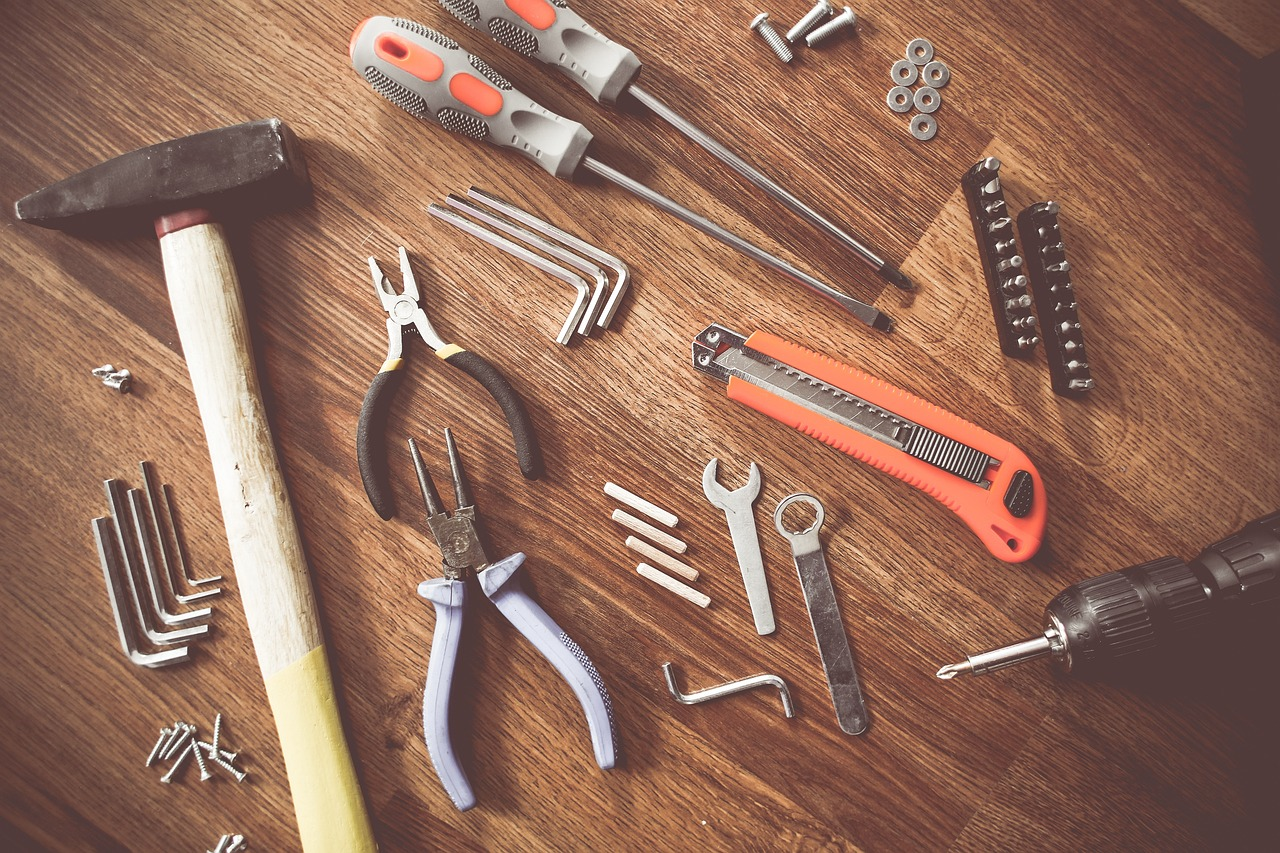
\includegraphics[height=0.8\textheight,trim={0 0 25cm 0},clip]{graphics/tools-864983_1280.jpg}         
                    \caption*{\href{https://pixabay.com/de/photos/werkzeuge-konstruieren-boot-864983/}{picjumbo\_com on pixabay}}    
                \end{flushleft}                
            \end{figure}
        \end{column} 
        \begin{column}{0.7\textwidth}
            Warum?
            \begin{itemize}[]
                \item Macht eure Daten überall verfügbar
                \item Erlaubt einfaches Teilen von Daten
            \end{itemize}
            Welche?
            \begin{itemize}[]
                \item Dropbox, Google Cloud, iCloud
                \item Sciebo
                \begin{itemize}
                    \item Sciebo: Die Hochschulcloud verfügbar an allen deutschen Hochschulen
                    \item Hostet in Deutschland
                    \item Kostenlose 30 GB
                \end{itemize}
            \end{itemize}
            Kriterien?
            \begin{itemize}[]
                \item $\geq$ 15 GB Speicherplatz
                \item Kostenlos
            \end{itemize}
        \end{column}        
    \end{columns}
\end{frame}

\begin{frame}[t]{Notizen}
    \begin{columns}[t]
        \begin{column}{0.29\textwidth}      
            \vspace{-3em} 
            \begin{figure}[t]
                \begin{flushleft}
                    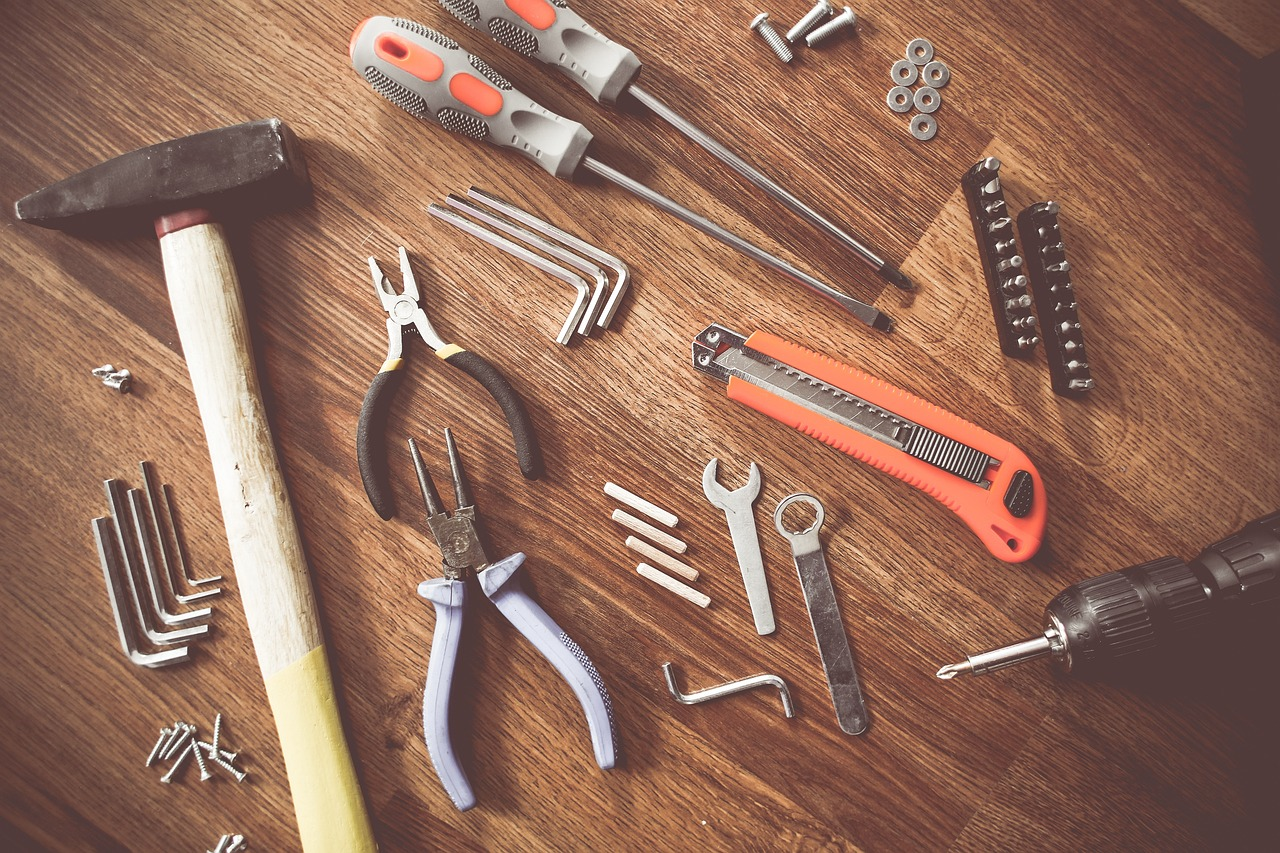
\includegraphics[height=0.8\textheight,trim={0 0 25cm 0},clip]{graphics/tools-864983_1280.jpg}         
                    \caption*{\href{https://pixabay.com/de/photos/werkzeuge-konstruieren-boot-864983/}{picjumbo\_com on pixabay}}    
                \end{flushleft}                
                      
            \end{figure}
        \end{column}        
        \begin{column}{0.7\textwidth}
            Welche?
            \begin{itemize}[]
                \item Google Docs, MS Word, Libre Office
                \item OneNote, Notion
                \item Obsidian, Joplin
            \end{itemize}
            Kriterien?
            \begin{itemize}[]
                \item Verfügbar auf allen Geräten
                \item Dateien übergreifende Suche
                \item Notizen verknüpfen
                \item Verknüpfungen zu Quellen herstellen
            \end{itemize}
        \end{column}
    \end{columns}
\end{frame}

\note{Ihr werdet immer eine Software brauchen, in der ihr Notizen anlegen könnt.
Word ist ein klassiker, aber nicht optimal für notizen.
OneNote ist ebenfalls von Microsoft, ist sehr flexibel, aber verwendet kein gängiges Format.
Joplin und Obsidian sind beides Tools die auf Markdown basieren.
Zusätzlich zu Notizen, müsst ihr die natürlich auch irgendwo Speichern, zusammen mit euren anderen Materialien.
Eine Cloud Lösung ist dafür ideal.
Dropbox ist eine der älteren und verbreiteten Lösungen. Sciebo ist eine alternative die von fast allen Universitäten angeboten wird. 
}



\subsection{Literatur}

\begin{frame}{Literatur Verwaltung}
    \begin{columns}[t]
        \begin{column}{0.39\textwidth}      
            \vspace{-2em} 
            \begin{figure}[t]
                \begin{flushleft}
                    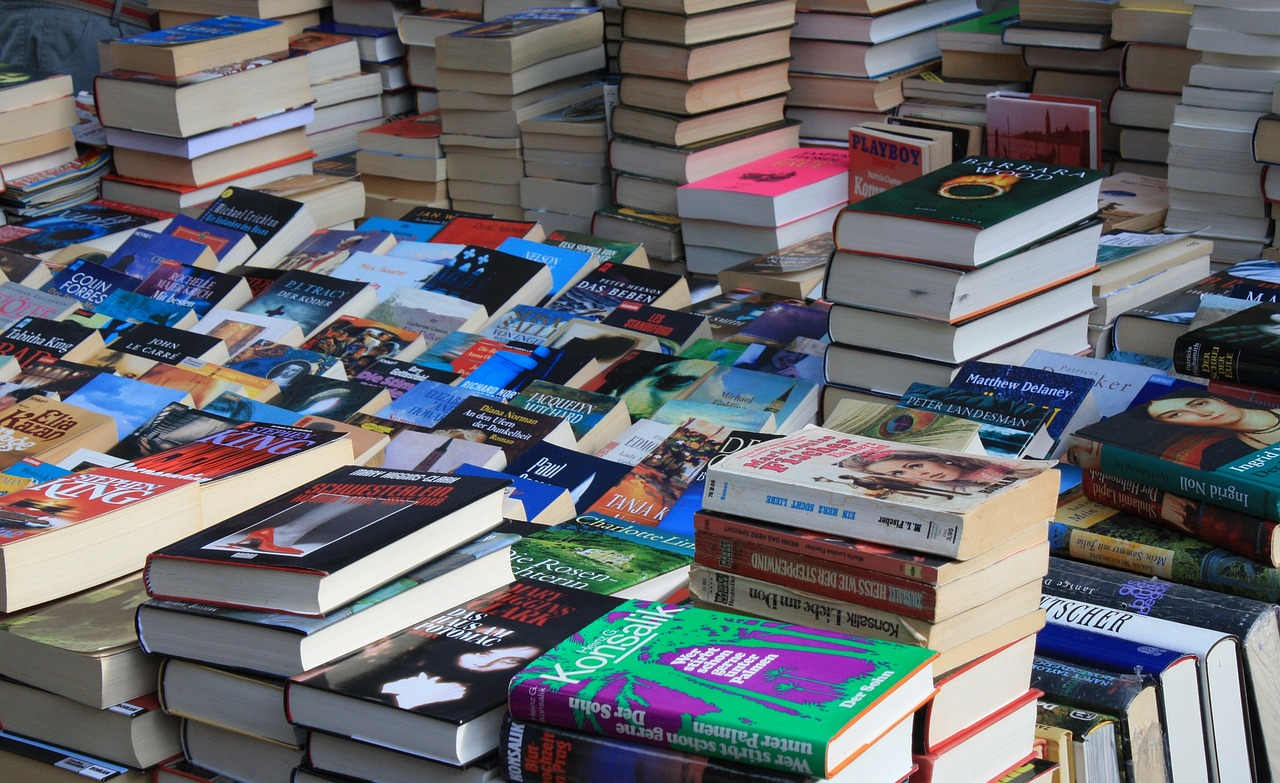
\includegraphics[height=0.8\textheight,trim={11cm 0 15cm 0},clip]{graphics/Flohmarkt.jpg}         
                    \caption*{\href{https://pixabay.com/de/photos/flohmarkt-bücher-kiste-stöbern-237460/}{geralt on pixabay}}    
                \end{flushleft}
            \end{figure}
        \end{column}          
        \begin{column}{0.69\textwidth}
            \begin{itemize}
                \item Citavi
                \item Mendeley
                \item Zotero
                \pause
                \begin{itemize}
                    \item Open Source
                    \item Kostenlos
                    \item Kompatibel mit MS Office, Google Docs and LaTeX
                    \item Features für PDF Annotation, Markieren und Notizen
                \end{itemize}
            \end{itemize}           
        \end{column}        
    \end{columns}    
\end{frame}

\begin{frame}{Literatur Recherche}
    \begin{columns}[t]
        \begin{column}{0.39\textwidth}      
            \vspace{-2em} 
            \begin{figure}[t]
                \begin{flushleft}
                    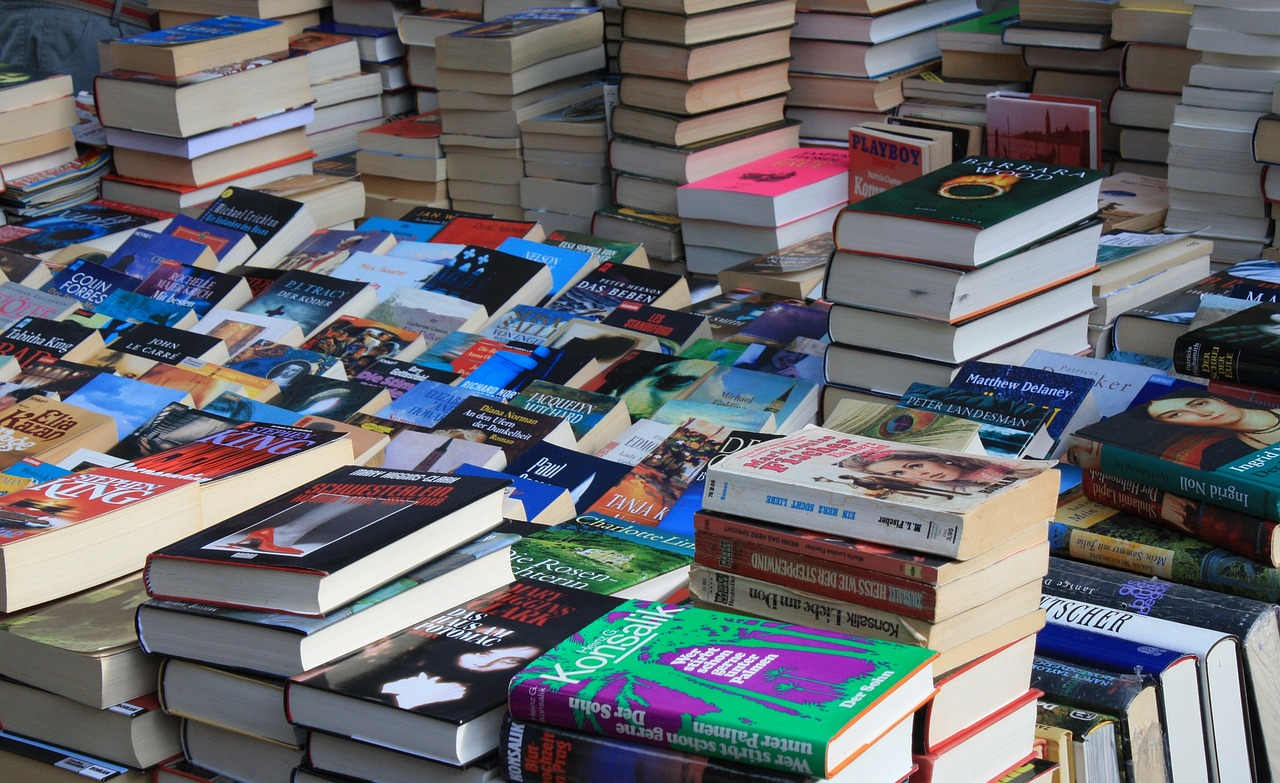
\includegraphics[height=0.8\textheight,trim={11cm 0 15cm 0},clip]{graphics/Flohmarkt.jpg}         
                    \caption*{\href{https://pixabay.com/de/photos/flohmarkt-bücher-kiste-stöbern-237460/}{geralt on pixabay}}    
                \end{flushleft}
            \end{figure}
        \end{column}        
        \begin{column}{0.69\textwidth}
            \begin{itemize}
                \item Google, \href{https://scholar.google.com/}{Google Scholar}
                \item \href{https://www.connectedpapers.com/}{Connected Papers}
                \item \href{https://elicit.com/}{Elicit}
                \item ChatGPT
                \item Eure Uni Bibliothek!
            \end{itemize}           
            \vspace{1cm}            
            \begin{itemize}
                \item \textcolor{lightgray}{libgen.ist}
                \item \textcolor{lightgray}{scihub.st}
            \end{itemize} 
        \end{column}        
    \end{columns}  
\end{frame}

\begin{frame}{Andere Materialien}
    \begin{columns}[t]
        \begin{column}{0.39\textwidth}      
            \vspace{-2em} 
            \begin{figure}[t]
                \begin{flushleft}
                    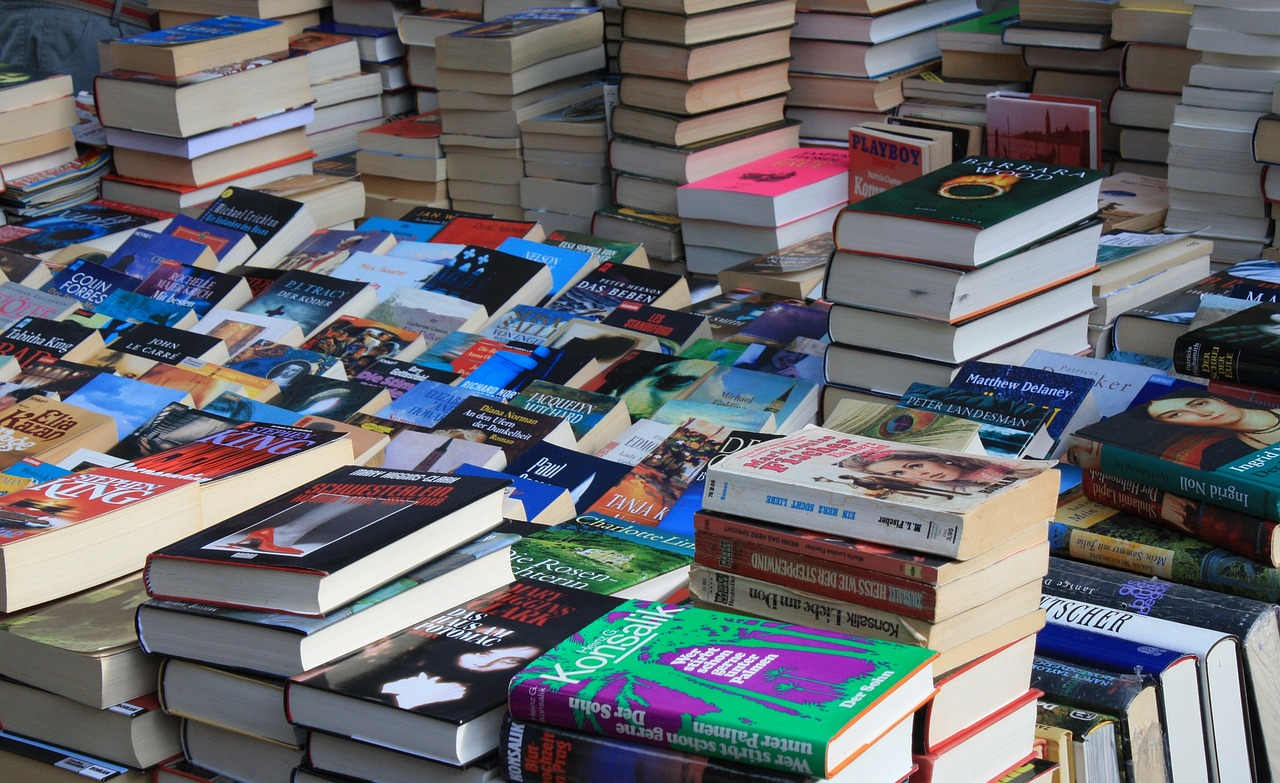
\includegraphics[height=0.8\textheight,trim={11cm 0 15cm 0},clip]{graphics/Flohmarkt.jpg}         
                    \caption*{\href{https://pixabay.com/de/photos/flohmarkt-bücher-kiste-stöbern-237460/}{geralt on pixabay}}    
                \end{flushleft}
            \end{figure}
        \end{column}          
        \begin{column}{0.69\textwidth}
            \begin{itemize}
                \item Hörbücher
                \begin{itemize}
                    \item LibriVox, Audible 
                \end{itemize}
                \item Bilder \& Grafiken
                \begin{itemize}
                    \item Google Bilder, Pixabax, Pexels
                \end{itemize}
                \item Vorlagen
                \begin{itemize}
                    \item Powerpoint: AllPPT.com
                    \item \LaTeX: Overleaf.com
                \end{itemize}

            \end{itemize}           
        \end{column}        
    \end{columns}    
\end{frame}

\begin{frame}[t]{Schreiben}
    \begin{columns}[t]
        \begin{column}{0.29\textwidth}      
            \vspace{-3em} 
            \begin{figure}[t]
                \begin{flushleft}
                    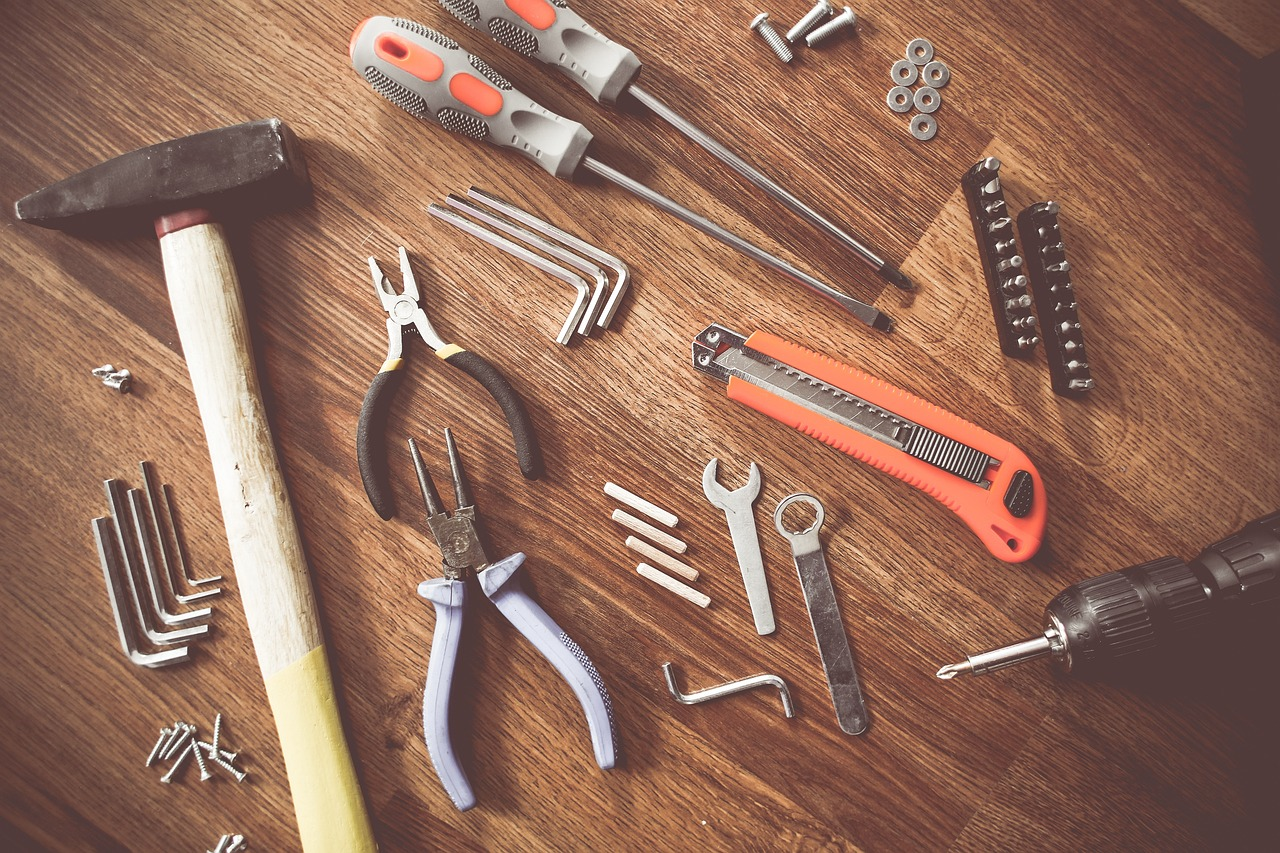
\includegraphics[height=0.8\textheight,trim={0 0 25cm 0},clip]{graphics/tools-864983_1280.jpg}         
                    \caption*{\href{https://pixabay.com/de/photos/werkzeuge-konstruieren-boot-864983/}{picjumbo\_com on pixabay}}    
                \end{flushleft}                
                      
            \end{figure}
        \end{column}        
        \begin{column}{0.7\textwidth}
            Welche?
            \begin{itemize}[]
                \item Google Docs, MS Word, Libre Office Write
                \item \LaTeX
                \item Markdown
            \end{itemize}
            Kriterien?
            \begin{itemize}[]
                \item Hochwertiger Output (PDF)
                \item Einfaches Referenzieren von Quellen
                \item Automatische Inhaltverzeichnisse
            \end{itemize}
        \end{column}
    \end{columns}
\end{frame}

\begin{frame}[t]{Präsentieren}
    \begin{columns}[t]
        \begin{column}{0.29\textwidth}      
            \vspace{-3em} 
            \begin{figure}[t]
                \begin{flushleft}
                    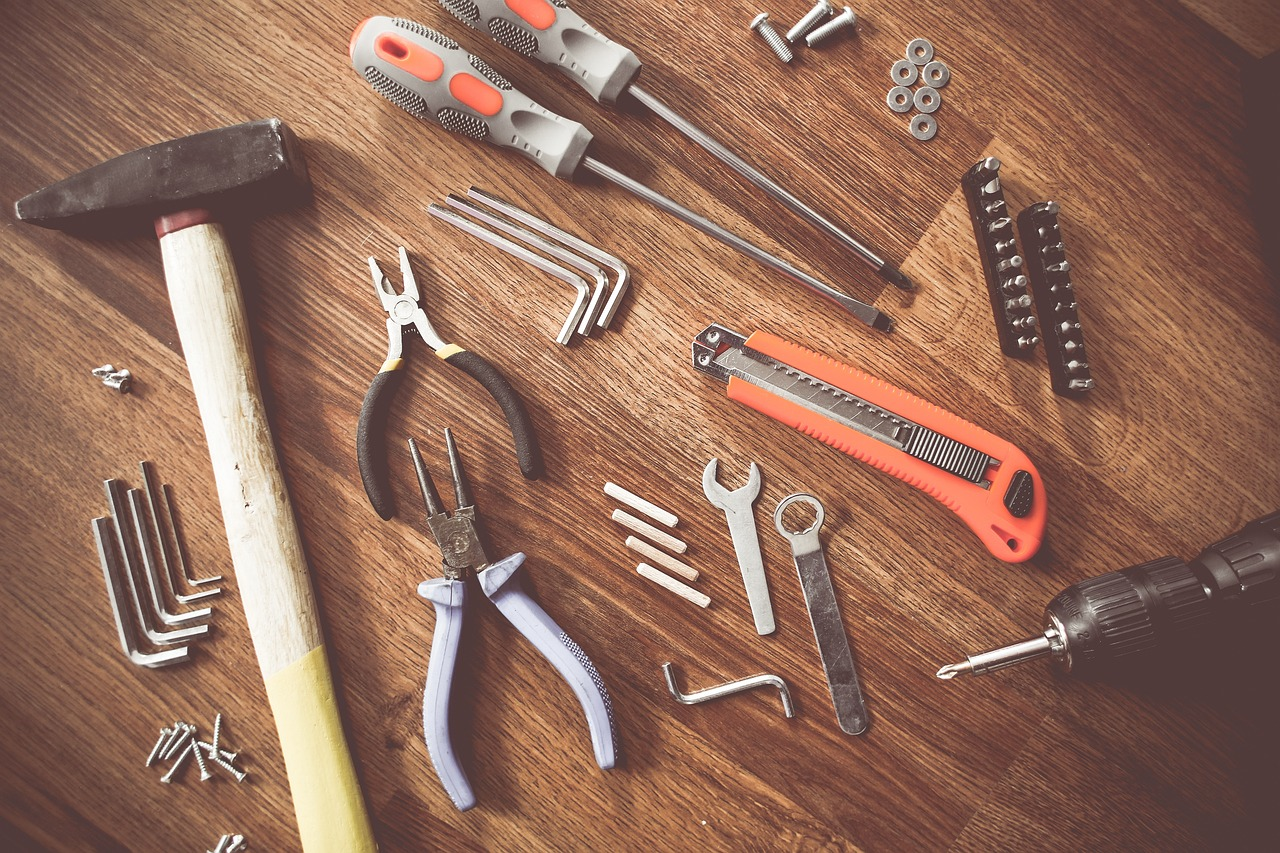
\includegraphics[height=0.8\textheight,trim={0 0 25cm 0},clip]{graphics/tools-864983_1280.jpg}         
                    \caption*{\href{https://pixabay.com/de/photos/werkzeuge-konstruieren-boot-864983/}{picjumbo\_com on pixabay}}    
                \end{flushleft}                
                      
            \end{figure}
        \end{column}        
        \begin{column}{0.7\textwidth}
            Welche?
            \begin{itemize}[]
                \item Google Slides, PowerPoint, LibreOffice Präsentationen
                \item \LaTeX
                \item Markdown
            \end{itemize}
            Kriterien?
            \begin{itemize}[]
                \item Hochwertiger Output
            \end{itemize}
        \end{column}
    \end{columns}
\end{frame}

\begin{frame}{Rechtschreibung und Gramatik}
    \begin{columns}[t]
        \begin{column}{0.4\textwidth}
            \vspace{-2em} 
            \begin{figure}
                \begin{flushleft}
                    
\includegraphics[height=0.6\textheight,trim={8cm 10 2cm 0},clip]{graphics/correcting-1870721_1280.jpg}
                    \caption*{\href{https://pixabay.com/photos/correcting-proof-paper-correction-1870721/}{3844328 on pixabay}}    
                \end{flushleft}                
            \end{figure}
            
        \end{column}
        \begin{column}{0.6\textwidth}
            \begin{itemize}
                \item Grammarly
                \item DudenMentor
                \item LanguageTool
                \begin{itemize}
                    \item Plugins für gängige Browser
                    \item Auch in der freien Version sehr mächtig
                \end{itemize}
            \end{itemize}
        \end{column}
    \end{columns}
\end{frame}

\begin{frame}[t]{Mein Tipp: Text Dateien}
    \begin{columns}[t]
        \begin{column}{0.29\textwidth}      
            \vspace{-3em} 
            \begin{figure}[t]
                \begin{flushleft}
                    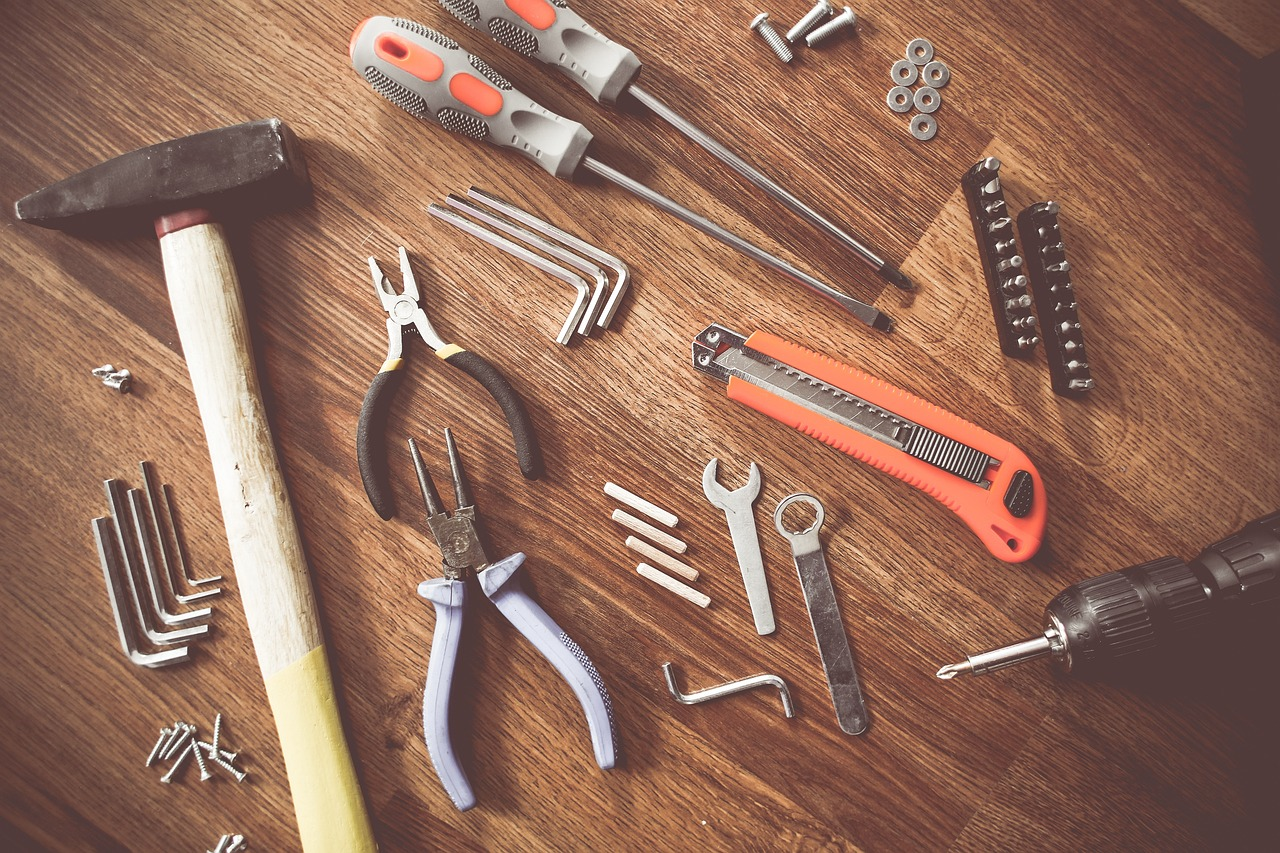
\includegraphics[height=0.8\textheight,trim={0 0 25cm 0},clip]{graphics/tools-864983_1280.jpg}         
                    \caption*{\href{https://pixabay.com/de/photos/werkzeuge-konstruieren-boot-864983/}{picjumbo\_com on pixabay}}    
                \end{flushleft}                
                      
            \end{figure}
        \end{column}        
        \begin{column}{0.7\textwidth}
            Plain Text
            \begin{itemize}
                \item ist portabel
                \item ist kompakt
                \item ist leicht zu durchsuchen
                \item einfach zu verwalten
            \end{itemize}
        \end{column}
    \end{columns}
\end{frame}


\begin{frame}{GIT}
    \begin{columns}
        \begin{column}{0.4\textwidth}
            \begin{flushleft}
                \begin{figure}
                    
\includegraphics[height=0.8\textheight]{graphics/final.jpg}
                \end{figure}    
            \end{flushleft}            
        \end{column}
        \begin{column}[t]{0.6\textwidth}
            \pause
            \vspace{-4cm}
            \begin{itemize}[]
                \item GIT
                \begin{itemize}
                    \item Erlaubt inkrementelles Verändern von Dateien
                    \item Gibt euch eine Historie aller Änderugen
                    \item Und eine Zeitmaschiene
                \end{itemize}
                \item Aber hat eine steile Lernkurve
            \end{itemize}
            
        \end{column}
    \end{columns}
\end{frame}


\begin{frame}{Gute Notizen sind nur die halbe Miete. }
    \begin{columns}
        \begin{column}{0.4\textwidth}
            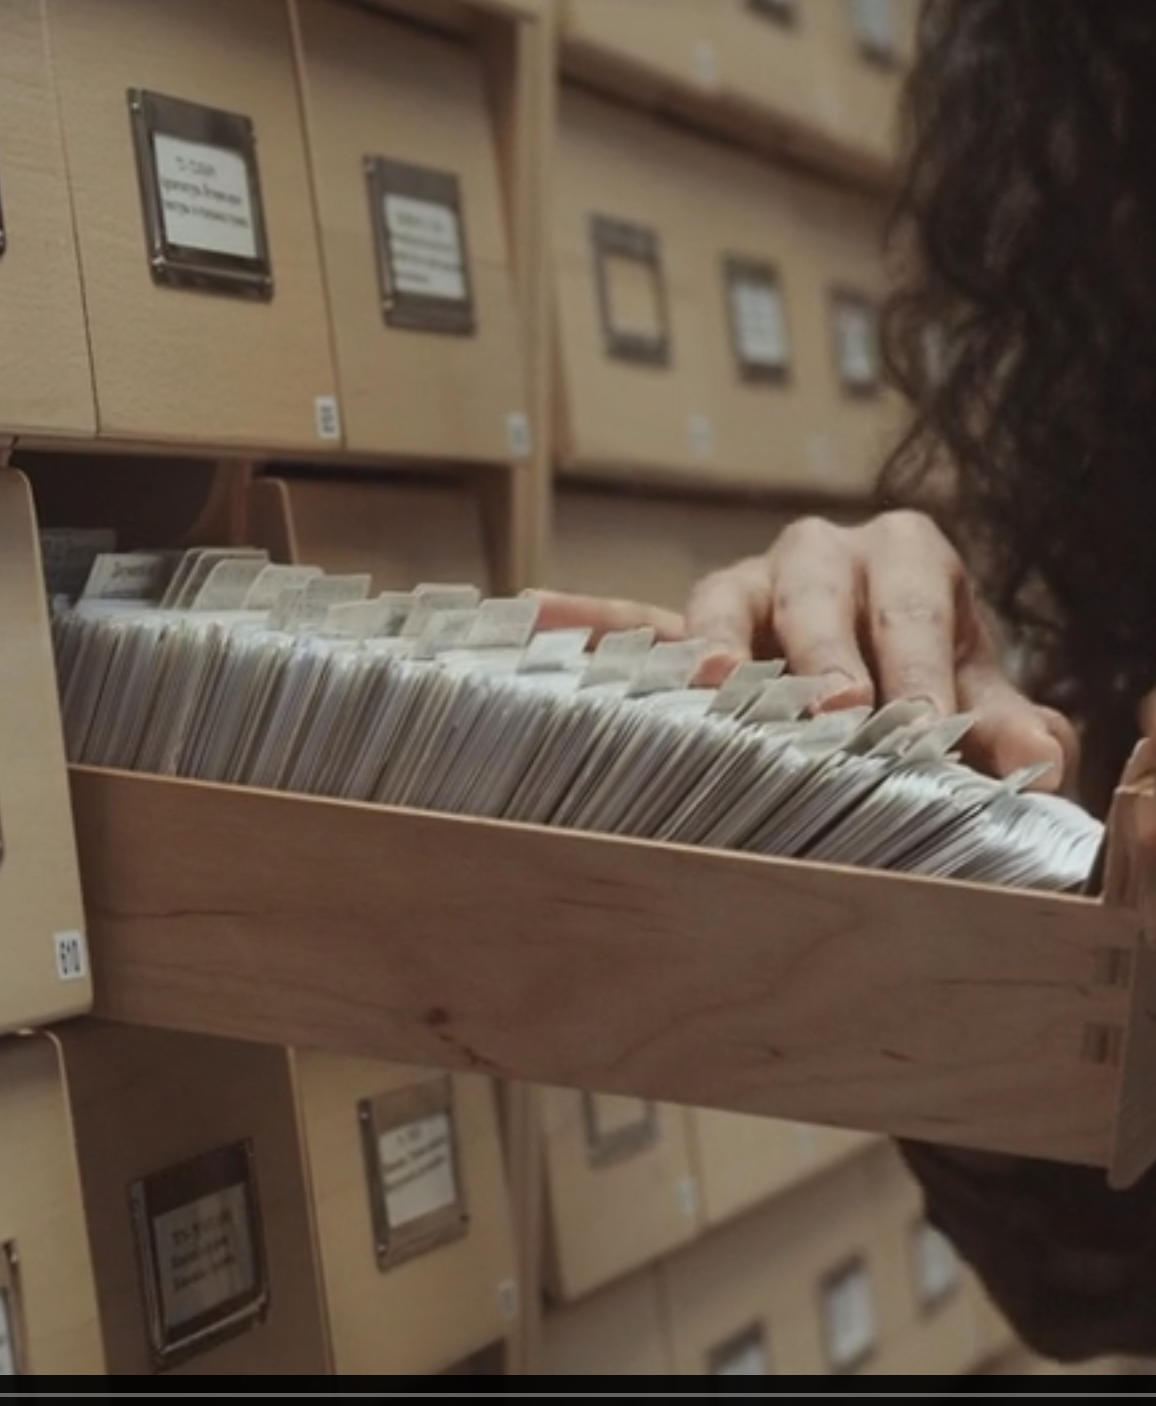
\includegraphics[width=\textwidth]{graphics/Zettelkasten.png}
        \end{column}
        \begin{column}[t]{0.6\textwidth}   
            \vspace{-3.5cm}
            \begin{block}{Der Zettelkasten}
                Eine gute Methode daraus anhaltendes Wissen zu generieren.
                \begin{itemize}
                    \item Atomare Notizen
                    \item Verlinkte Notizen
                    \item Frage/Antwort Zettel
                \end{itemize} 
            \end{block}                     
        \end{column}        
    \end{columns}    
\end{frame}

\begin{frame}{Gute Notizen sind nur die halbe Miete}
    \begin{columns}
        \begin{column}{0.4\textwidth}
            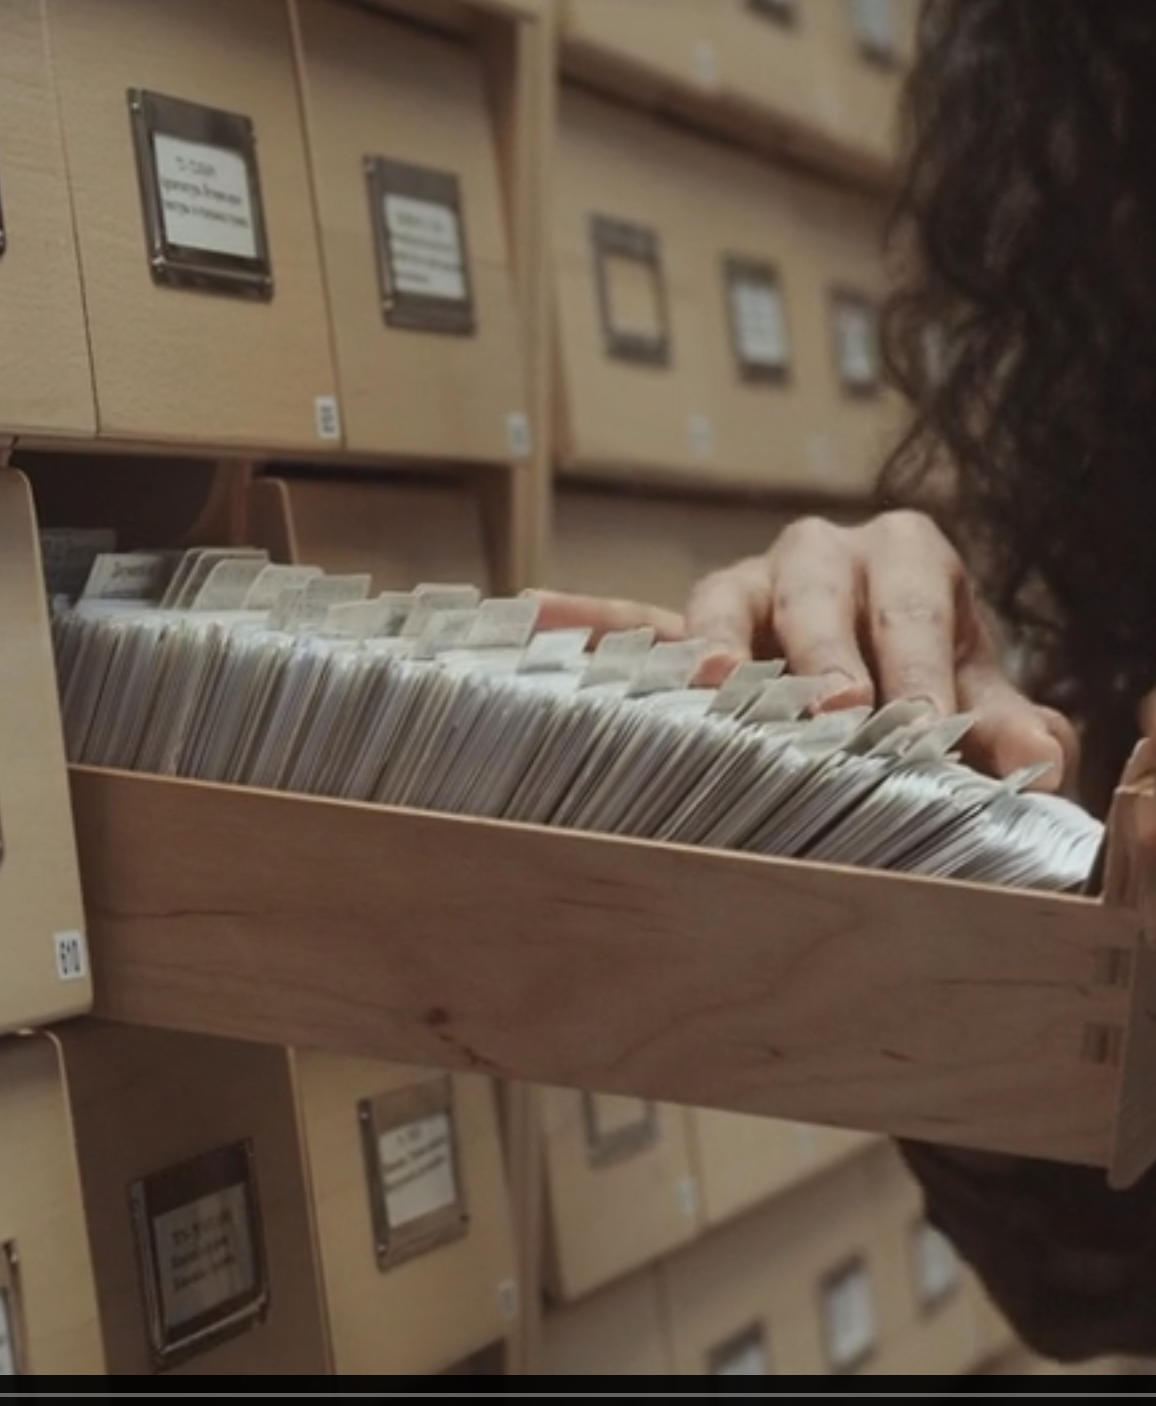
\includegraphics[width=\textwidth]{graphics/Zettelkasten.png}
        \end{column}
        \begin{column}[t]{0.6\textwidth} 
            \vspace{-4cm}
            \begin{figure}[h]
                
\includegraphics[width=\textwidth]{graphics/Logos/anki.png}
            \end{figure}  
            \begin{block}{Karteikarten mit Anki}
                Einfaches Erstellen von Lernkarten
                Clients für PC/Mac und Android/iOS
                
            \end{block}                     
        \end{column}        
    \end{columns}    
\end{frame}

\begin{frame}{Gute Notizen sind nur die halbe Miete}
    \begin{columns}
        \begin{column}{0.4\textwidth}
            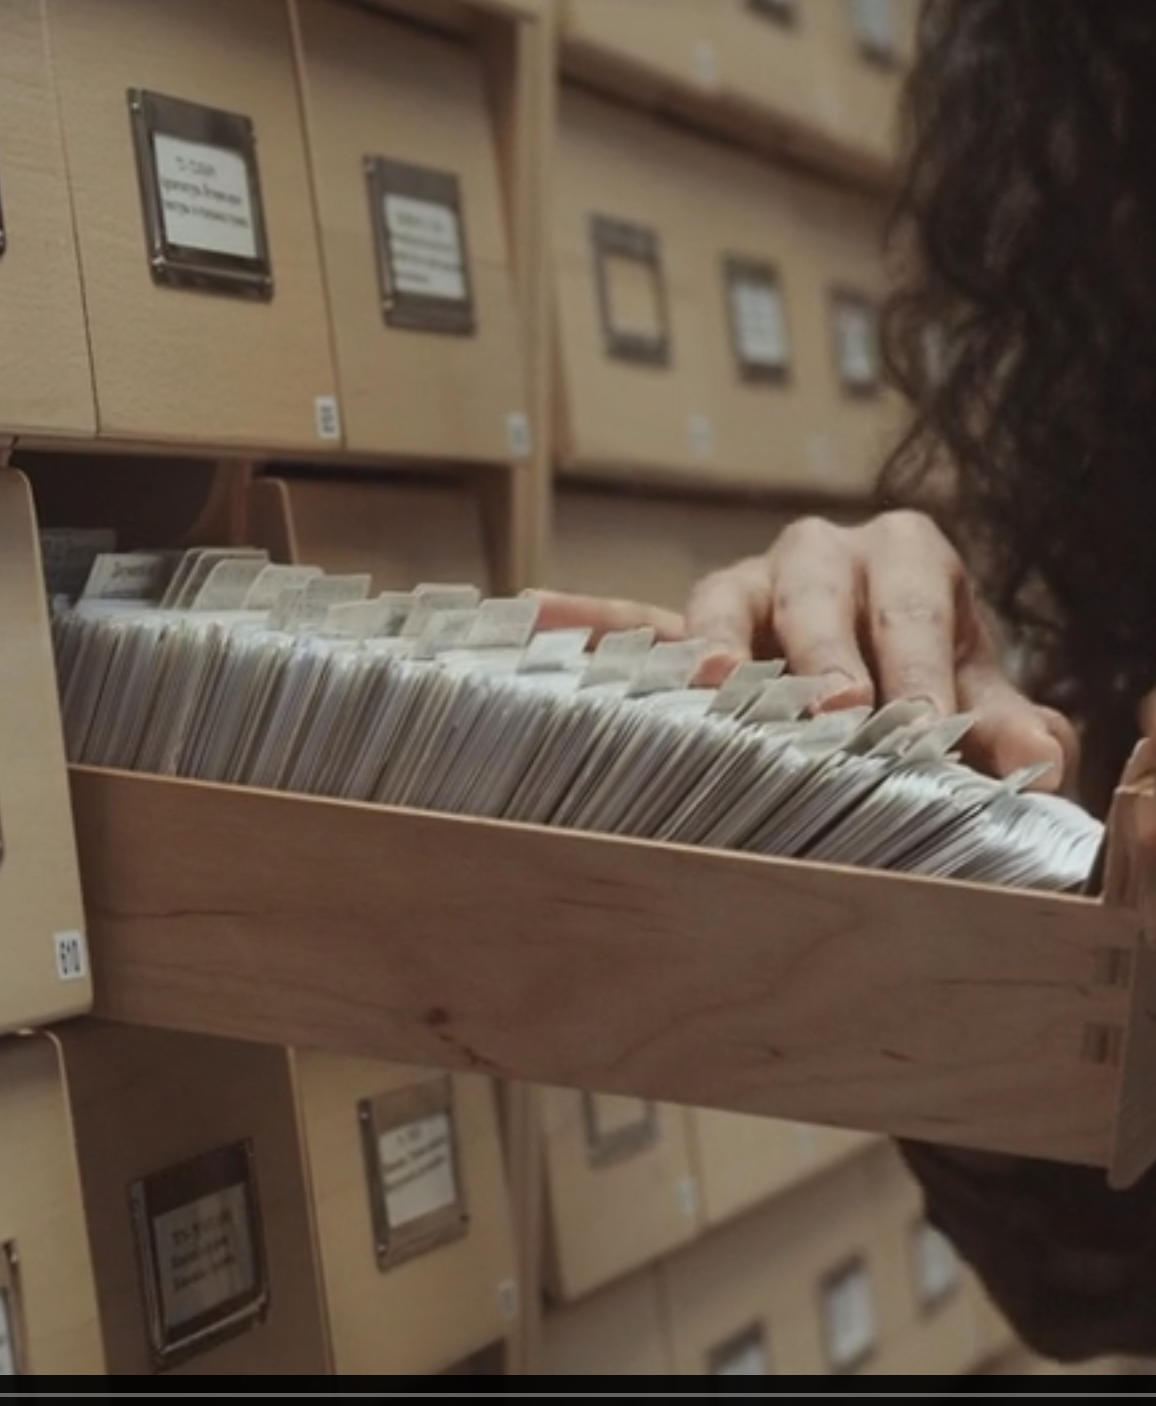
\includegraphics[width=\textwidth]{graphics/Zettelkasten.png}
        \end{column}
        \begin{column}[t]{0.6\textwidth}
            \vspace{-3cm}
            \begin{itemize}[]
                \item Mindmaps
                \begin{itemize}
                    \item Excalidraw
                    \item freeplan.com
                \end{itemize}
                \item Visualisierung
                \begin{itemize}
                    \item \href{https://explaineverything.com/}{Explain Everything}
                    \item \href{https://www.drawio.com/}{Drawio}
                \end{itemize}
            \end{itemize} 


            
        \end{column}        
    \end{columns}    
\end{frame}

\begin{frame}{Kommunikation}
    \begin{columns}[t]
        \begin{column}{0.4\textwidth}
            \vspace{-2em} 
            \begin{figure}
                \begin{flushleft}
                    
\includegraphics[height=0.8\textheight,trim={4cm 0 17cm 0},clip]{graphics/call-2946023_1280.jpg}
                    \caption*{\href{https://pixabay.com/photos/call-afro-megaphone-scream-symbol-2946023/}{fietzfotos on pixabay}}    
                \end{flushleft}                
            \end{figure}            
        \end{column}
        \begin{column}{0.6\textwidth}
            \begin{itemize}
                \item WhatsApp, Telegram
                \item Slack
                \item Matrix        
                \item Discord
                \begin{itemize}
                    \item Kostenlos
                    \item Unterstützt Text, Voice und Video Chats
                    \item Gruppen ermöglichen Organistion der Kommunikation
                \end{itemize}    
            \end{itemize}
        \end{column}
    \end{columns}
\end{frame}

\begin{frame}{Kommunikation}
    \begin{columns}[t]
        \begin{column}{0.4\textwidth}
            \vspace{-2em} 
            \begin{figure}
                \begin{flushleft}
                    
\includegraphics[height=0.8\textheight,trim={4cm 0 17cm 0},clip]{graphics/call-2946023_1280.jpg}
                    \caption*{\href{https://pixabay.com/photos/call-afro-megaphone-scream-symbol-2946023/}{fietzfotos on pixabay}}    
                \end{flushleft}                
            \end{figure}            
        \end{column}
        \begin{column}{0.6\textwidth}
            Communities:
            \begin{itemize}
                \item Reddit 
                \begin{itemize}
                    \item Communities zu methoden, Fächern und Tools mit vielen hilfsbereiten Mitgliedern
                \end{itemize} 
                \item YouTube 
                \item Discord Server
                \begin{itemize}
                    \item Hard zu finden, aber ein guter Interaktionsort für spezifische Themen.
                \end{itemize}        
            \end{itemize}
        \end{column}
    \end{columns}
\end{frame}


\subsection{Ordnung}
\begin{frame}[t]{Dateien Ordentlich ablegen}
    \begin{columns}
        \begin{column}{0.5\textwidth}
            \vspace{-6cm}
            \begin{block}{Ein paar Grundregeln}
                \begin{itemize}
                    \item Überlegt euch eine Struktur.                 
                    \item Versucht möglichst wenige Ordner Level zu haben.
                    \item Schreibt eure Struktur auf. Gute Angewohnheit: Eine ReadMe in den Top Ordner legen.
            \end{itemize}  
            \end{block}
            {\small Ein paar Quellen:
            \begin{itemize}[]
                \item \href{https://www.youtube.com/watch?v=WtKeeDYA_2I&t=317s}{YouTube}
                \item \href{https://ocw.mit.edu/courses/res-str-002-data-management-spring-2016/497580bd31c004cc758a2afb0a115aa4_MITRES_STR_002S16_File.pdf}{MIT Open Courseware}
            \end{itemize}
            }

            \vfill   
        \end{column}
        \begin{column}[t]{0.5\textwidth}
            \begin{forest}
                for tree={
                    font=\ttfamily,
                    grow'=0,
                    child anchor=west,
                    parent anchor=south,
                    anchor=west,
                    calign=first,
                    inner xsep=7pt,
                    s sep=1pt,
                    edge path={
                    \noexpand\path [draw, \forestoption{edge}]
                    (!u.south west) +(2pt,0) |- (.child anchor) pic {folder} \forestoption{edge label};
                    },
                    file/.style={edge path={\noexpand\path [draw, \forestoption{edge}]
                    (!u.south west) +(7.5pt,0) |- (.child anchor) \forestoption{edge label};},
                    inner xsep=2pt,inner ysep=0pt,font=\small\ttfamily
                            },
                    before typesetting nodes={
                    if n=1
                        {insert before={[,phantom]}}
                        {if n=3 
                        {insert before={[,phantom]}}
                        {}
                        }                
                    },
                    fit=band,
                    before computing xy={l=15pt},
                }  
                [SS24
                    [ReadMe.txt,file]
                    [Grundlagen 1
                        [SW1
                            [VL.pdf,file]
                            [Übung.pdf,file]
                        ]
                        [SW2]
                    ]
                    [Nebenfach 1
                        [VL
                            [VL1.pdf,file]
                            [VL2.pdf,file]
                        ]
                        [Übungen
                            [Ü1.pdf,file]
                            [Ü2.pdf,file]
                        ]
                    ]
                ]
                \end{forest}
        \end{column}
    \end{columns}
\end{frame}

\subsection{Zeitmanagement}

\begin{frame}{Stundenplan}
    \begin{figure}
       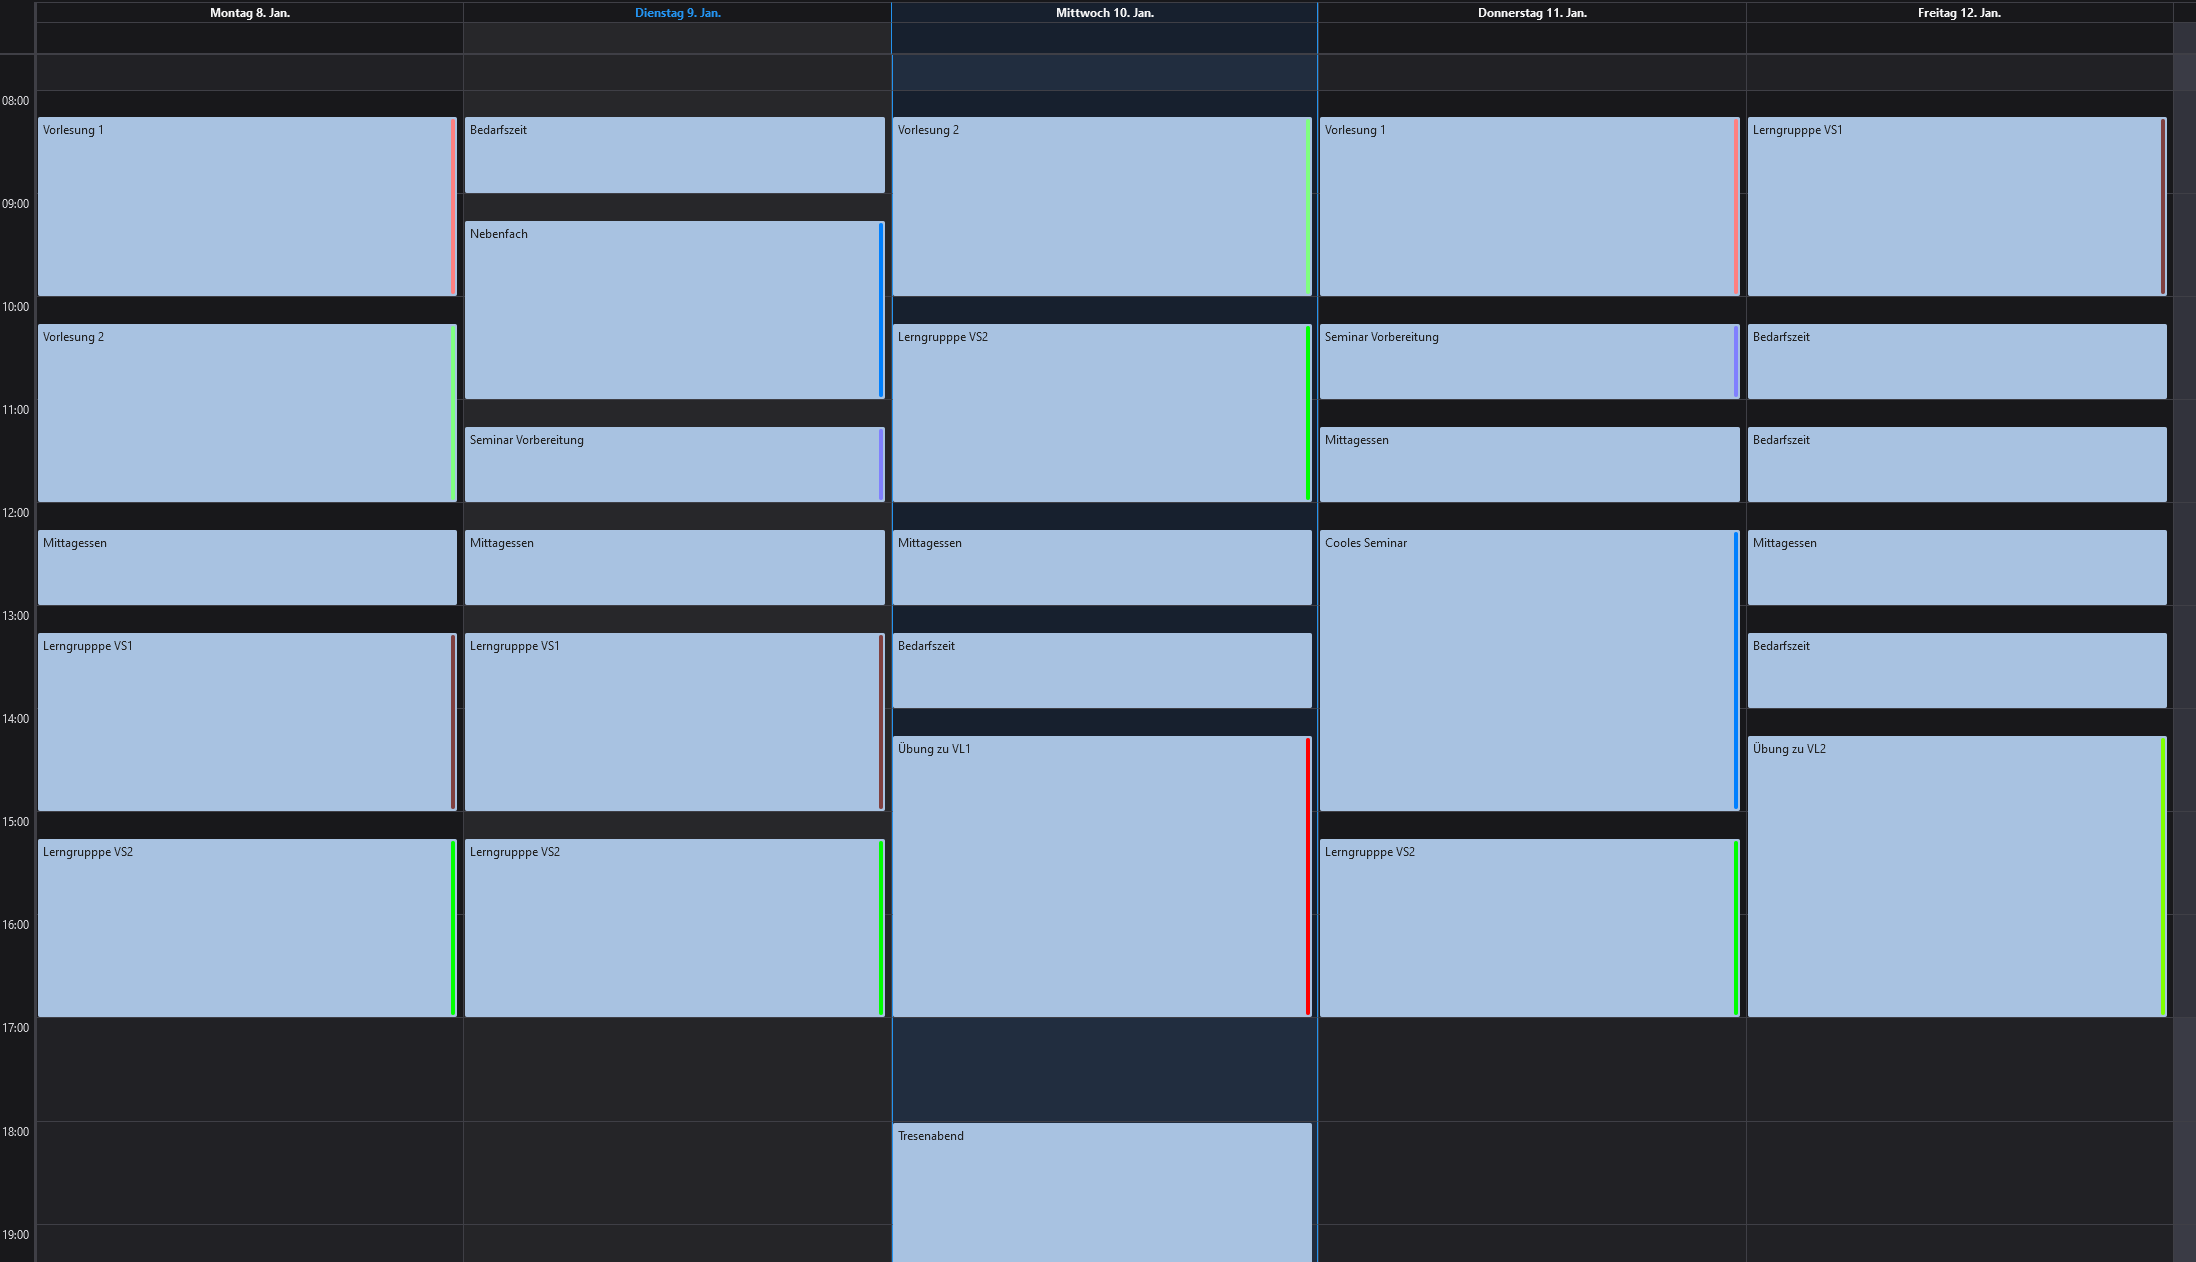
\includegraphics[width=0.8\textwidth]{graphics/Kalender/Kalender5.PNG};
    \end{figure}
\end{frame}

\begin{frame}{Time Boxing}    
    \begin{figure}
       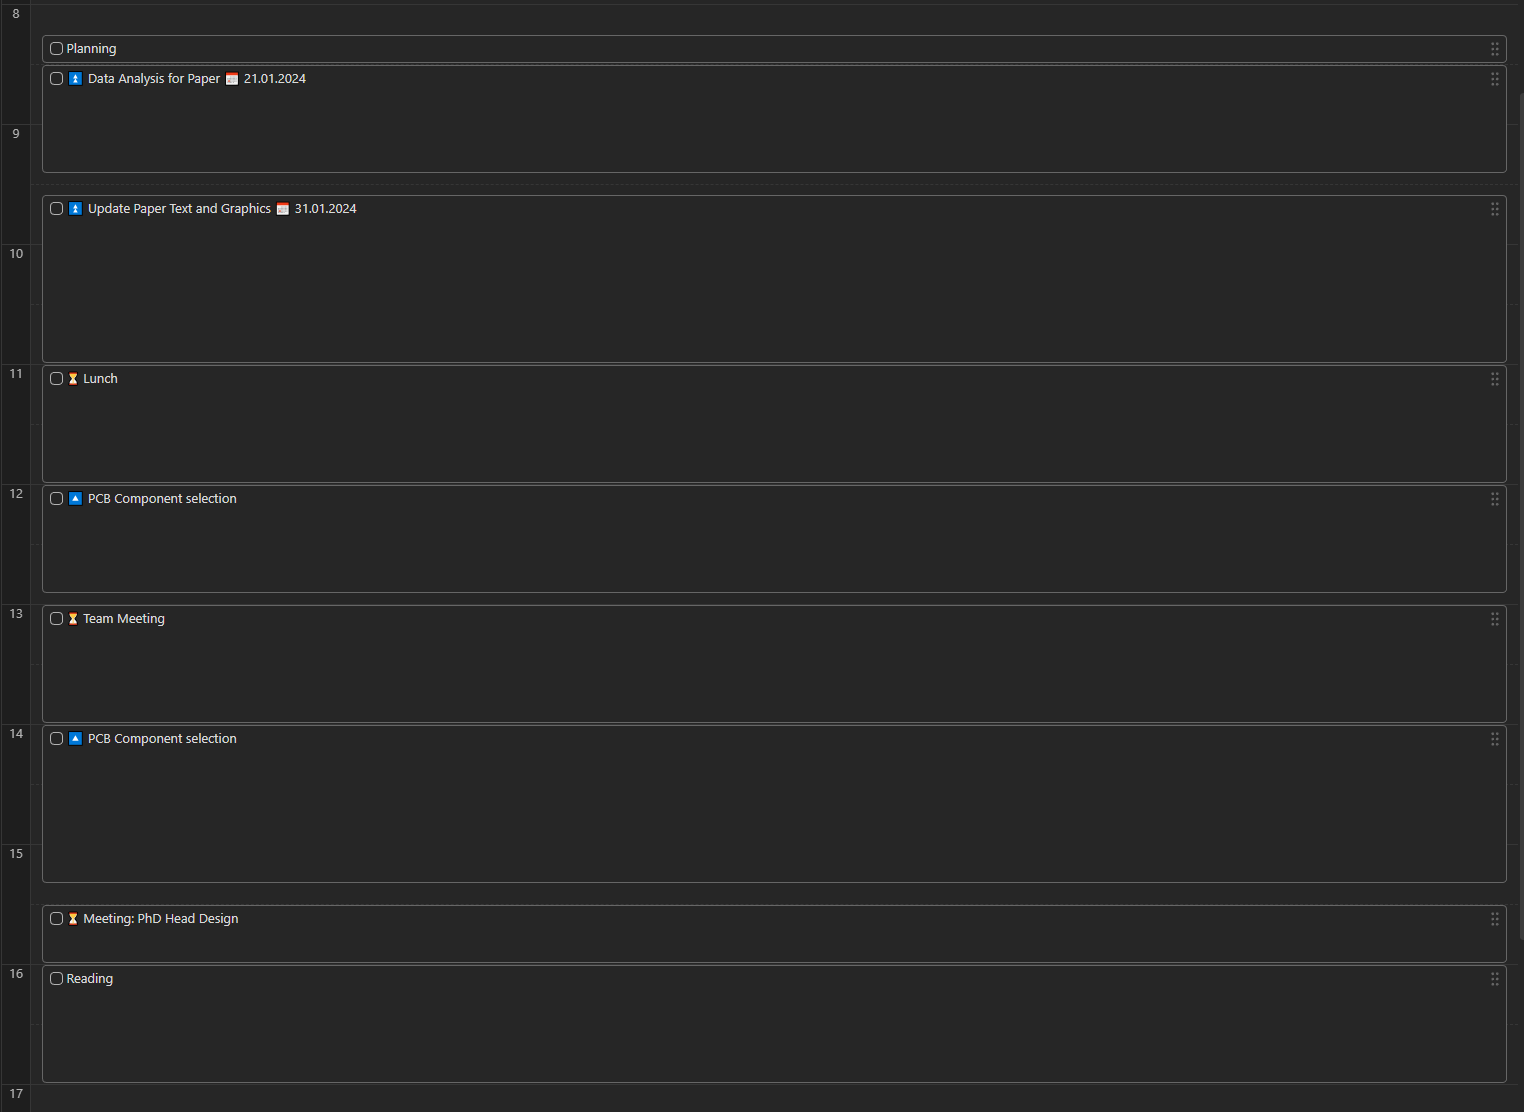
\includegraphics[height=0.8\textheight,trim={0 0 10cm 0},clip]{graphics/MyDailyPlan.png};
    \end{figure}
\end{frame}
\note{
Kalender       
Pomodoro}

\begin{frame}{Mehr Ansätze:}
    \begin{columns}[t]
        \begin{column}{0.3\textwidth}
            \begin{figure}
                \begin{flushleft}
                    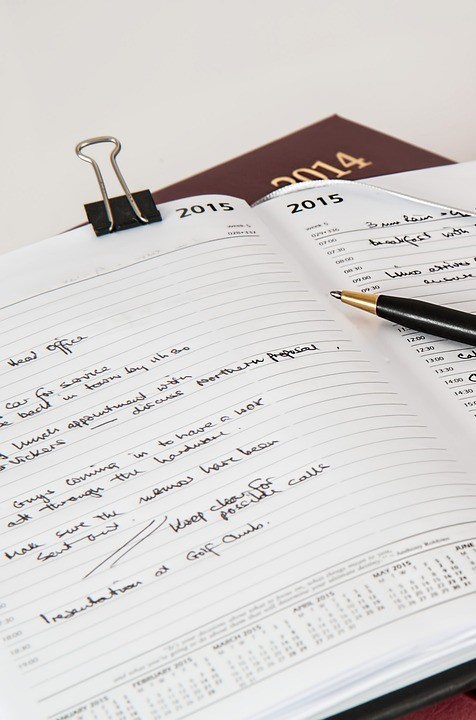
\includegraphics[width=\textwidth]{graphics/diary-614149_960_720.jpg}
                    \caption*{\href{https://pixabay.com/de/photos/tagebuch-stift-notizbuch-januar-614149/}{stevepb on pixabay}}    
                \end{flushleft}                
            \end{figure}
            
        \end{column}
        \begin{column}{0.7\textwidth}
            \begin{itemize}
                \item ToDo Listen
                \begin{itemize}
                    \item \href{https://to-do.office.com/tasks/}{Microsoft ToDo}
                    \item \href{https://todoist.com/de}{todoist}
                    \item \dots
                \end{itemize}
                \item Pomodoro Technik
                \item \begin{itemize}
                    \item \href{https://pomofocus.io/}{Pomofocus}
                    \item \dots
                \end{itemize}                 
            \end{itemize}
        \end{column}
    \end{columns}
\end{frame}


\begin{frame}{Und noch mehr}
    \begin{columns}[t]
    \begin{column}{0.49\textwidth}
        \begin{figure}
            \begin{flushleft}
                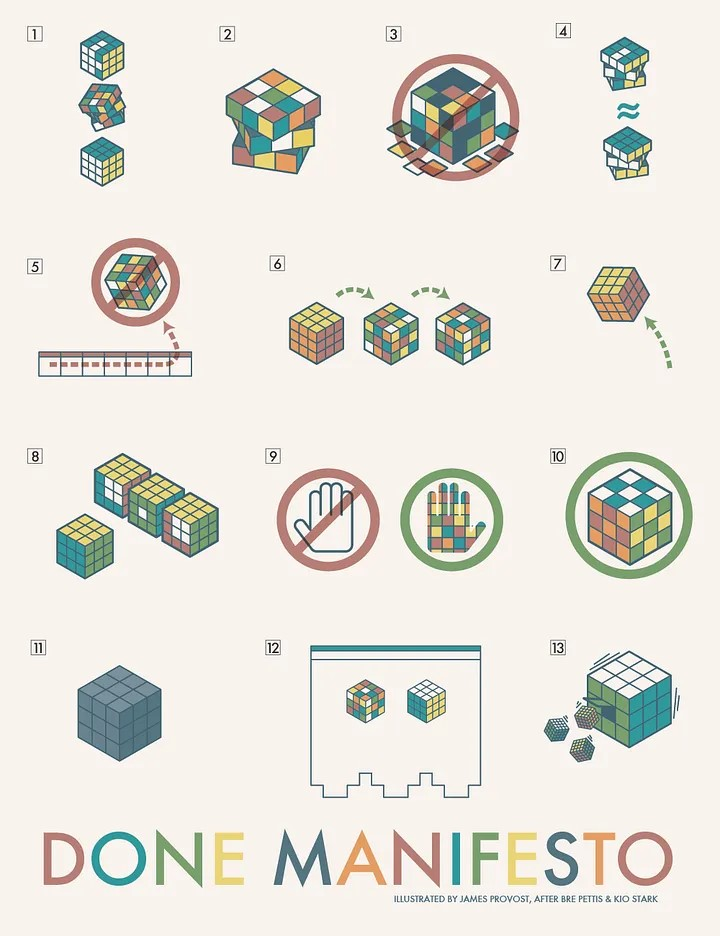
\includegraphics[height=0.7\textheight]{graphics/TheDoneManifesto.jpg}
                \caption*{\href{https://medium.com/@bre/the-cult-of-done-manifesto-724ca1c2ff13}{The Done Manifesto}}   
            \end{flushleft}                
        \end{figure}        
    \end{column}
    \begin{column}{0.49\textwidth}
        \begin{figure}
            \begin{flushleft}
                
\includegraphics[height=0.7\textheight]{graphics/GTD.png}
                \caption*{\href{https://www.thalia.de/shop/home/artikeldetails/A1052684525?ProvID=11000731&msclkid=add9b427aa0c13222c40d1b812e94a42&gclsrc=ds}{David Allen Getting Things Done}}    
            \end{flushleft}                
        \end{figure}        
    \end{column}
\end{columns}
\end{frame}



\begin{frame}{Honorable Mentions}
    \begin{columns}[t]
        \begin{column}{0.4\textwidth}
            \vspace{-2em} 
            \begin{figure}
                \begin{flushleft}
                    
\includegraphics[height=0.8\textheight,trim={4cm 0 17cm 0},clip]{graphics/winner-1548239_1280.jpg}
                    \caption*{\href{https://pixabay.com/photos/winner-medal-gold-award-success-1548239/}{AxxLC on pixabay}}    
                \end{flushleft}                
            \end{figure}            
        \end{column}
        \begin{column}{0.6\textwidth}
            \begin{itemize}
                \item Online Lern Plattformen
                \begin{itemize}
                    \item \href{https://ocw.mit.edu/}{MIT Open Coureseware}
                \end{itemize}  
                \item Tree Style Tabs Browser Plugins
                \begin{itemize}
                    \item Organisiert Browsertabs besser
                \end{itemize}  
                \item Passwort Manager
                \begin{itemize}
                    \item Generell eine gute Empfehlung
                \end{itemize}  
                \item GitHub
                \begin{itemize}
                    \item Eine Gute Quelle und eine gute Möglichkeit zum Online Stellen von Material
                \end{itemize} 
                \item \LaTeX  
            \end{itemize}
        \end{column}
    \end{columns}
\end{frame}

\begin{frame}{Themen über die wir sonst noch reden können}
    \begin{columns}
        \begin{column}{0.6\textwidth}
            \begin{itemize}
                \item Wie komme ich an einen günstigen Laptop?
                \item Wie Google ich richtig?
                \item Exkurse
                \begin{itemize}
                    \item in mein Notiz System: Obsidian
                    \item in meine Zotero Bibliothek
                \end{itemize} 
            \end{itemize}
        \end{column}
        \begin{column}{0.4\textwidth}
            \begin{figure}
                \begin{flushleft}
                    
\includegraphics[width=\textwidth,trim={0 0 0 0},clip]{graphics/QRCode.png}
                \end{flushleft}                
            \end{figure}               
        \end{column}
    \end{columns}
\end{frame}

\section{Addendum}
\begin{frame}{Ein Laptop für den schmalen Euro}
    \begin{columns}
        \begin{column}{0.6\textwidth}
            \begin{figure}
                \begin{flushleft}
                    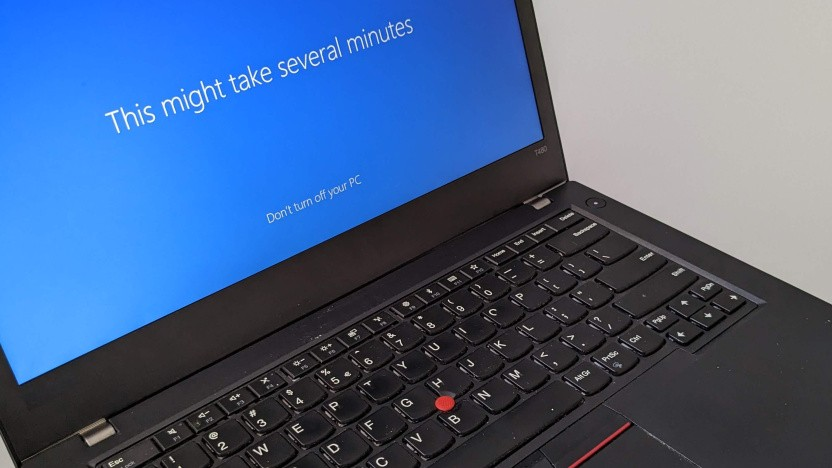
\includegraphics[width=\textwidth,trim={0 0 0 0},clip]{graphics/ThinkPad.jpg}
                \end{flushleft}                
            \end{figure} 
        \end{column}
        \begin{column}{0.4\textwidth}
            \begin{itemize}
                \item ThinkPad T480
                \begin{itemize}
                    \item Robust und einfach abzugraden
                    \item Gebraucht für 150€
                    \item Ersatz Akku für 150€
                    \item 1 TB SSD für 60€
                \end{itemize} 
                \item Laptop Powerbank für 100€
                \item Betriebssystem: Ubuntu für 0€
            \end{itemize}
            \href{https://www.golem.de/news/diy-mein-thinkpad-t480-ist-so-gut-wie-ein-macbook-air-m1-2308-176569.html}{[Quelle]}
        \end{column}
    \end{columns}
\end{frame}

\begin{frame}{Ein kurzer Google Cheat Sheet}
    \begin{itemize}
        \item \textit{site:} beschränke die Suche auf eine Webseite
        \item \textit{filetype:} sucht nach Dateien vom Typ
        \item \textit{""}  Muss im Ergebnis vorkommen
        \item \textit{-} Darf nicht im Ergebnis vorkommen
        \item \textit{AND,OR} Logisches Verknüpfen von Suchbegriffen
    \end{itemize}
\end{frame}

\end{document}